% A LaTeX template for MSc Thesis submissions to 
% Politecnico di Milano (PoliMi) - School of Industrial and Information Engineering
%
% S. Bonetti, A. Gruttadauria, G. Mescolini, A. Zingaro
% e-mail: template-tesi-ingind@polimi.it
%
% Last Revision: October 2021
%
% Copyright 2021 Politecnico di Milano, Italy. NC-BY

\documentclass{Configuration_Files/PoliMi3i_thesis}

%------------------------------------------------------------------------------
%	REQUIRED PACKAGES AND  CONFIGURATIONS
%------------------------------------------------------------------------------

% CONFIGURATIONS
\usepackage{parskip} % For paragraph layout
\usepackage{setspace} % For using single or double spacing
\usepackage{emptypage} % To insert empty pages
\usepackage{multicol} % To write in multiple columns (executive summary)
\setlength\columnsep{15pt} % Column separation in executive summary
\setlength\parindent{10pt} % Indentation
\raggedbottom  

% PACKAGES FOR TITLES
\usepackage{titlesec}
% \titlespacing{\section}{left spacing}{before spacing}{after spacing}
\titlespacing{\section}{0pt}{3.3ex}{2ex}
\titlespacing{\subsection}{0pt}{3.3ex}{1.65ex}
\titlespacing{\subsubsection}{0pt}{3.3ex}{1ex}
\usepackage{color}

% PACKAGES FOR LANGUAGE AND FONT
\usepackage[english]{babel} % The document is in English  
\usepackage[utf8]{inputenc} % UTF8 encoding
\usepackage[T1]{fontenc} % Font encoding
\usepackage[11pt]{moresize} % Big fonts

% PACKAGES FOR IMAGES
\usepackage{graphicx}
\usepackage{svg}
\usepackage{transparent} % Enables transparent images
\usepackage{eso-pic} % For the background picture on the title page
%\usepackage{subfig} % Numbered and caption subfigures using \subfloat.
\usepackage[export]{adjustbox}
\usepackage{tikz} % A package for high-quality hand-made figures.
\usetikzlibrary{}
\graphicspath{{./Images/}} % Directory of the images
\usepackage{caption} % Coloured captions
\usepackage{subcaption}
\usepackage{xcolor} % Coloured captions
\usepackage{amsthm,thmtools,xcolor} % Coloured "Theorem"
\usepackage{float}

% STANDARD MATH PACKAGES
\usepackage{amsmath}
\usepackage{amsthm}
\usepackage{amssymb}
\usepackage{amsfonts}
\usepackage{bm}
\usepackage{cancel}
\usepackage[overload]{empheq} % For braced-style systems of equations.
\usepackage{fix-cm} % To override original LaTeX restrictions on sizes

% PACKAGES FOR TABLES
\usepackage{tabularx}
\usepackage{longtable} % Tables that can span several pages
\usepackage{colortbl}
\usepackage{multicol} % added by Simone

% PACKAGES FOR ALGORITHMS (PSEUDO-CODE)
\usepackage{algorithm}
\usepackage{algorithmic}

% PACKAGES FOR REFERENCES & BIBLIOGRAPHY
\usepackage[colorlinks=true,linkcolor=black,anchorcolor=black,citecolor=black,filecolor=black,menucolor=black,runcolor=black,urlcolor=black]{hyperref} % Adds clickable links at references
\usepackage{cleveref}
\usepackage[square, numbers, sort&compress]{natbib} % Square brackets, citing references with numbers, citations sorted by appearance in the text and compressed
\bibliographystyle{plain} % You may use a different style adapted to your field

% OTHER PACKAGES
\usepackage{pdfpages} % To include a pdf file
\usepackage{afterpage}
\usepackage{lipsum} % DUMMY PACKAGE
\usepackage{fancyhdr} % For the headers
\usepackage{fancyvrb}
\usepackage[acronym]{glossaries}
\usepackage{enumitem} 
\fancyhf{}
\usepackage[utf8]{inputenc}
\usepackage{geometry}
\geometry{a4paper, margin=1in}
\usepackage{booktabs}
\usepackage{tabularx}

% PACKAGES FOR ALLOY
\usepackage[dvipsnames]{xcolor}
\usepackage{listings}
\usepackage{alloy-style}

% Input of configuration file. Do not change config.tex file unless you really know what you are doing. 
% Define blue color typical of polimi
\definecolor{bluepoli}{cmyk}{0.4,0.1,0,0.4}
\definecolor{Green}{RGB}{30, 170, 0}

% Custom theorem environments
\declaretheoremstyle[
  headfont=\color{bluepoli}\normalfont\bfseries,
  bodyfont=\color{black}\normalfont\itshape,
]{colored}

% Set-up caption colors
%\captionsetup[figure]{labelfont={color=bluepoli}} % Set colour of the captions
%\captionsetup[table]{labelfont={color=bluepoli}} % Set colour of the captions
%\captionsetup[algorithm]{labelfont={color=bluepoli}} % Set colour of the captions
\captionsetup{font=bf}

\theoremstyle{colored}
\newtheorem{theorem}{Theorem}[chapter]
\newtheorem{proposition}{Proposition}[chapter]
\newtheorem{definition}{Definition}[chapter]

% Enhances the features of the standard "table" and "tabular" environments.
\newcommand\T{\rule{0pt}{2.6ex}}
\newcommand\B{\rule[-1.2ex]{0pt}{0pt}}

% Pseudo-code algorithm descriptions.
\newcounter{algsubstate}
\renewcommand{\thealgsubstate}{\alph{algsubstate}}
\newenvironment{algsubstates}
  {\setcounter{algsubstate}{0}%
   \renewcommand{\STATE}{%
     \stepcounter{algsubstate}%
     \Statex {\small\thealgsubstate:}\space}}
  {}

% New font size
\newcommand\numfontsize{\@setfontsize\Huge{200}{60}}

% Title format: chapter
\titleformat{\chapter}[hang]{
\fontsize{50}{20}\selectfont\bfseries\filright}{\textcolor{bluepoli} \thechapter\hsp\hspace{2mm}\textcolor{bluepoli}{|   }\hsp}{0pt}{\huge\bfseries \textcolor{bluepoli}
}

% Title format: section
\titleformat{\section}
{\normalfont\Large\bfseries}
{\thesection.}{1em}{}
%{\color{bluepoli}\normalfont\Large\bfseries}
%{\color{bluepoli}\thesection.}{1em}{}

% Title format: subsection
\titleformat{\subsection}
{\normalfont\large\bfseries}
{\thesubsection.}{1em}{}
%{\color{bluepoli}\normalfont\large\bfseries}
%{\color{bluepoli}\thesubsection.}{1em}{}

% Title format: subsubsection
\titleformat{\subsubsection}
{\normalfont\bfseries}
{\thesubsubsection.}{1em}{}
%{\color{bluepoli}\normalfont\large\bfseries}
%{\color{bluepoli}\thesubsubsection.}{1em}{}

% Shortening for setting no horizontal-spacing
\newcommand{\hsp}{\hspace{0pt}}

\makeatletter
% Renewcommand: cleardoublepage including the background pic
\renewcommand*\cleardoublepage{%
  \clearpage\if@twoside\ifodd\c@page\else
  \null
  \AddToShipoutPicture*{\BackgroundPic}
  \thispagestyle{empty}%
  \newpage
  \if@twocolumn\hbox{}\newpage\fi\fi\fi}
\makeatother

%For correctly numbering algorithms
\numberwithin{algorithm}{chapter}

%----------------------------------------------------------------------------
%	NEW COMMANDS DEFINED
%----------------------------------------------------------------------------

% EXAMPLES OF NEW COMMANDS
\newcommand{\bea}{\begin{eqnarray}} % Shortcut for equation arrays
\newcommand{\eea}{\end{eqnarray}}
\newcommand{\e}[1]{\times 10^{#1}}  % Powers of 10 notation

%----------------------------------------------------------------------------
%	ADD YOUR PACKAGES (be careful of package interaction)
%----------------------------------------------------------------------------

%----------------------------------------------------------------------------
%	ADD YOUR DEFINITIONS AND COMMANDS (be careful of existing commands)
%----------------------------------------------------------------------------

\makeglossaries

\newacronym{acronym}{ACR}{Acronym}

%----------------------------------------------------------------------------
%	BEGIN OF YOUR DOCUMENT
%----------------------------------------------------------------------------

\begin{document}

\fancypagestyle{plain}{%
\fancyhf{} % Clear all header and footer fields
% \fancyhead[RO,RE]{\thepage} %RO=right odd, RE=right even
\fancyhead[R]{\thepage} % R=right
\renewcommand{\headrulewidth}{0pt}
\renewcommand{\footrulewidth}{0pt}}

%----------------------------------------------------------------------------
%	TITLE PAGE
%----------------------------------------------------------------------------

\pagestyle{empty} % No page numbers
\frontmatter % Use roman page numbering style (i, ii, iii, iv...) for the preamble pages

\puttitle{
	title=Requirement Analysis and Specification Document \\ \textit{Students\&Companies}, % Title of the thesis
	name=
	Russolillo Simone \\
	Visani Valeria Benedetta Cecilia\\
	Wang Toni, % Author Name and Surname
	course=Software Engineering II \\ Computer Science and Engineering, % Study Programme (in Italian)
	ID  =
	11100725 \\
	10730247 \\
	10817365,  % Student ID number (numero di matricola)
	% advisor= Prof. Name Surname, % Supervisor name
	% coadvisor={}, % Co-Supervisor name, remove this line if there is none
	academicyear={2024-25},  % Academic Year
} % These info will be put into your Title page 

%----------------------------------------------------------------------------
%	PREAMBLE PAGES: ABSTRACT (inglese e italiano), EXECUTIVE SUMMARY
%----------------------------------------------------------------------------

% \pagebreak
% \pagestyle{empty}
% \hspace{0pt}
% \vfill
% \textit{Dedicated to my family.}
% \vfill
% \hspace{0pt}
% \pagebreak

% \startpreamble
% \setcounter{page}{1} % Set page counter to 1

% % ABSTRACT IN ENGLISH
% \chapter*{Abstract} 
% Here goes the abstract.
% \\
% \\
% \textbf{Keywords:} key, words, go, here% Keywords

% % ABSTRACT IN ITALIAN
% \chapter*{Abstract in lingua italiana}
% Qui va inserito l'abstract in italiano.
% \\
% \\
% \textbf{Parole chiave:} qui, vanno, le, parole, chiave% Keywords (italian)

%----------------------------------------------------------------------------
%	LIST OF CONTENTS/FIGURES/TABLES/SYMBOLS
%----------------------------------------------------------------------------

% TABLE OF CONTENTS
\thispagestyle{empty}
\tableofcontents % Table of contents 
\thispagestyle{empty}
\cleardoublepage

%-------------------------------------------------------------------------
%	THESIS MAIN TEXT
%-------------------------------------------------------------------------
% In the main text of your thesis you can write the chapters in two different ways:
%
%(1) As presented in this template you can write:
%    \chapter{Title of the chapter}
%    *body of the chapter*
%
%(2) You can write your chapter in a separated .tex file and then include it in the main file with the following command:
%    \chapter{Title of the chapter}
%    \input{chapter_file.tex}
%
% Especially for long thesis, we recommend you the second option.

\addtocontents{toc}{\vspace{2em}} % Add a gap in the Contents, for aesthetics
\mainmatter % Begin numeric (1,2,3...) page numbering

% --------------------------------------------------------------------------
% NUMBERED CHAPTERS % Regular chapters following
% --------------------------------------------------------------------------

\chapter{Introduction}

\section{Purpose}

\section{Scope}
\subsection{World Phenomena}
\subsection{Machine Phenomena}
\subsection{Shared Phenomena}

\section{Definitions, Acronyms, Abbreviations}
\subsection{Definitions}
\subsection{Acronyms}
\subsection{Abbreviations}

\section{Reference Documents}

\section{Document Structure} % Introduction
\chapter{Architectural Design}

% //////////////////////////////
% ------------------------------
\section{Overview}
% ------------------------------
% //////////////////////////////

% //////////////////////////////
% ------------------------------
\subsection{High Level View}
% ------------------------------
% //////////////////////////////

This section provides an overview of the architectural components that make up the Students\&Companies system and highlights their key interactions.

The Students\&Companies system adopts a microservices architectural approach. This style of architecture involves designing the application as a collection of independent services, each responsible for a specific functionality. These services collaborate with one another to fulfill the system's overall objectives. To enhance clarity, a high-level representation of the system, including its microservices, is shown in the following image:

% ---------------------------------
% ---------------------------------
% IMAGE
\vspace{20pt}
\hrule
\vspace{10pt}
IMAGE
\vspace{10pt}
\hrule
\vspace{20pt}
% IMAGE
% ---------------------------------
% ---------------------------------

From a high-level viewpoint, the elements mentioned earlier are illustrated in the figure below. At the top, the client is represented by the first icon, while the Students\&Companies system is depicted as a collection of microservices. \textcolor{red}{At the bottom of the figure}, the data layer is represented with a database icon.

The Students\&Companies system comprises several microservices, each fulfilling specific responsibilities. Their details are as follows:

\begin{itemize}
    \item \textbf{Gateway Microservice:} This microservice manages two key functionalities. Firstly, it handles the authentication process for users, such as students, companies, and universities. All incoming user requests are processed by the Gateway, which dispatches them to the relevant microservice for handling. Similarly, all system responses are routed back through the Gateway to reach the users. To ensure scalability and performance, this microservice can be replicated on the server side.

    \item \textbf{User Management Microservice:} Responsible for managing user data and profiles, this microservice oversees the profiles of students, companies, and universities. It provides user profile pages and ensures seamless access to personal data whenever required.

    \item \textbf{Recommendation System Microservice:} This microservice is tasked with analyzing student CVs, company project details, and internship data to recommend suitable matches between students and companies. It uses algorithms and data from the shared database to optimize the pairing process.

    \item \textbf{Internship Management Microservice:} This microservice handles all aspects of internships. It supports the creation and updating of internship listings, manages student applications, and provides detailed views of ongoing and completed internships.

    \item \textbf{Selection Process Management Microservice:} Dedicated to assisting in the selection and recruitment process, this microservice provides features such as managing interview schedules, handling offer confirmations, and finalizing internship agreements.

    \item \textbf{Communication Platform Microservice:} This microservice facilitates communication between students, companies, and universities. It provides a dedicated platform for exchanging messages, addressing inquiries, and resolving internship-related issues.

    \item \textbf{Feedback\&Complaint Microservice:} Focused on gathering and managing feedback, this microservice enables users to submit complaints or reviews about internships. It provides tools for universities to monitor and address reported issues effectively.

    \item \textbf{Notification Microservice:} Responsible for managing notifications throughout the system, this microservice listens to events (event-driven architecture) and sends timely alerts to users, such as internship deadlines, application updates, or system announcements.

    \item \textbf{Statistical Analysis Tool:} This tool aids in analyzing historical data and user feedback to refine the recommendation algorithms and improve the overall user experience.
\end{itemize}

As for the interactions between these microservices, they will be elaborated upon in greater detail in the subsequent sections of this document. For now, it is important to highlight that all communications between the client and the Students\&Companies platform are routed through the Gateway Microservice. Additionally, the various user interfaces provided by the platform are supplied by different microservices, each handling the data and functionalities specific to their domain. However, the delivery of these interfaces to the client is always mediated by the gateway.

All microservices in the system expose \textbf{RESTful APIs}, which serve as the primary access points to their data and functionalities. When necessary, microservices interact with each other through these APIs, and the specifics of these interactions will be outlined in subsequent views.

Moreover, every microservice has access to a \textbf{shared database} via the interfaces provided by the DBMS. While all microservices share this common data space, each one is responsible for distinct operations and computations based on the specific functionalities it offers.

The system’s internal interactions are also built upon an \textbf{event-driven architecture}. In this pattern, microservices can asynchronously publish events to an Event Bus or Event Queue. Other components within the system can consume these events and perform actions in response. Further details regarding this architecture will be provided in the following sections of the Design Document.

% //////////////////////////////
% ------------------------------
\section{Component View}
% ------------------------------
% //////////////////////////////

This section aims to provide an overview of the various components that constitute the Students\&Companies system. UML Component diagrams are utilized to represent the logical software elements that work collaboratively to achieve the objectives defined for the development of the system.

Given that the structural components of the Students\&Companies platform cannot be effectively represented in a single diagram, multiple diagrams are presented. This approach is adopted to ensure clarity and avoid overcrowding the visualizations. The diagrams have been organized based on the principle of grouping components that frequently interact with one another.

It is worth noting that, despite the division into separate diagrams for explanation purposes, the system functions as a cohesive whole. The components depicted in these diagrams belong to the same system and collectively contribute to the overall operation and functionality of the platform.

% //////////////////////////////
% ------------------------------
\subsection{RESTful APIs Component Diagram}
% ------------------------------
% //////////////////////////////

One of the key features highlighted in the introductory section of the Students\&Companies project is that microservices provide RESTful APIs to handle incoming commands, share data, and interact with each other. This view focuses on outlining, from a broad perspective, how these microservices leverage their APIs to operate efficiently.

% ---------------------------------
% ---------------------------------
% IMAGE
\vspace{20pt}
\hrule
\vspace{10pt}
IMAGE
\vspace{10pt}
\hrule
\vspace{20pt}
% IMAGE
% ---------------------------------
% ---------------------------------

Let’s analyze the key concepts conveyed by the diagram. This UML component diagram is used to illustrate the RESTful APIs provided by each microservice within the Students\&Companies system. These APIs perform specific computations on data related to the functionality offered by the respective microservice. For example, the Internship Management Microservice exposes an API that processes internship data within the shared database and returns relevant internship information.

The Gateway Microservice serves as the entry point for all user requests. The Dispatcher component inside the Gateway is responsible for routing user requests to the appropriate microservices that are tasked with handling them. This explains why the Dispatcher "uses" all the APIs exposed by the other microservices.

In certain cases, the microservices in the Students\&Companies system may also interact with one another through their RESTful APIs to perform joint computations In this diagram, these interactions are shown. For
instance:

\begin{itemize}
    \item The Notification Microservice needs to query the Student Manager, University Manager, Company Manager inside the User Management Microservice whenever it needs to deliver the notification to a specific set of users.
    \item The Notification Microservice must query the User Management Microservice when the list of all students in the Students\&Companies system is required (for example, to notify all students about a new internship opportunity available on the platform).
    \item The Communication Platform Microservice uses the Notification API to deliver alerts such as internship status updates, interview invitations, or feedback to the appropriate users.
    \item The Recommendation System Microservice must leverage the Statistical Analysis Tool to refine its matching algorithms and provide better internship recommendations based on student profiles and internship data.
    \item The User Management Microservice uses the Internship Management API to update student profiles once they have been matched with an internship, ensuring that the students' records reflect their current opportunities.
    \item The Internship Management Microservice must interact with the Selection Process Management Microservice to facilitate the selection process, including interview scheduling and the finalization of student placements.
    \item The Feedback\&Complaint Microservice interacts with the Statistical Analysis Tool to provide useful information for recommendations.
\end{itemize}

This diagram must be interpreted considering the event-driven paradigm adopted in the Students\&Companies project. Some interactions and event flows within the system occur asynchronously, following an event-driven approach that is further explained in subsequent views. This is why certain interactions, which may appear absent here, are actually managed asynchronously to improve the overall system performance.

Another crucial aspect to highlight regarding this diagram is the "Manager" components within the various microservices. These components internally implement a Model-View-Controller pattern to deliver their services. The following representation illustrates a component diagram that focuses solely on the internals of the "Manager" component for a generic microservice:

% ---------------------------------
% ---------------------------------
% IMAGE
\vspace{20pt}
\hrule
\vspace{10pt}
IMAGE
\vspace{10pt}
\hrule
\vspace{20pt}
% IMAGE
% ---------------------------------
% ---------------------------------

The Model component is responsible for organizing and managing data. Each microservice in the Students\&Companies system is designed to handle a specific portion of the data domain. For example, the Internship Management Microservice focuses solely on managing and providing information about internships. Consequently, each Model component within the Manager components ensures data consistency with the DBMS, accessing it when necessary, and performing related operations.

The View component offers the user interface. Since different microservices handle various types of information within the Students\&Companies ecosystem, multiple user interfaces are distributed across the microservices and managed by their respective View components.

The Controller acts as the "bridge" between the Model and the View. This component is responsible for:
\begin{itemize}
    \item Receiving requests from the View component when the user interacts with the user interface.
    \item Performing the appropriate computation based on those requests.
    \item Manipulating data through the Model, passing user requests to the data layer.
    \item Updating the View if the computation results in changes to the user interface.
\end{itemize}

Throughout this document, the term "Manager" component will be used in a more general sense to encompass the behavior and functionality of this internal architecture.

% //////////////////////////////
% ------------------------------
\subsection{Service Discovery Component Diagram}
% ------------------------------
% //////////////////////////////

This simple component diagram illustrates an important service provided by the Gateway Microservice to allow all microservices to locate and collaborate with each other. This service is known as "Service Discovery" and involves maintaining a register (inside the Gateway Microservice) of active microservices.

In this way:
\begin{itemize}
    \item A newly launched microservice can register itself to be discovered by other microservices.
    \item All microservices can contact other active microservices in the system to send requests.
\end{itemize}

Here’s the diagram:

% ---------------------------------
% ---------------------------------
% IMAGE
\vspace{20pt}
\hrule
\vspace{10pt}
IMAGE
\vspace{10pt}
\hrule
\vspace{20pt}
% IMAGE
% ---------------------------------
% ---------------------------------

The interpretation is straightforward. The Gateway Microservice contains a component called the Discovery Service, which implements the logic to provide the discovery functionality. The Discovery Service component exposes an API (\texttt{DiscoveryServiceAPI}), which can be used by all other microservices to locate each other.

% //////////////////////////////
% ------------------------------
\subsection{Event-Driven Pattern Components}
% ------------------------------
% //////////////////////////////

This section illustrates all the components required to implement asynchronous, event-driven communication between microservices in the system. This design decision has been made to optimize the system, particularly for interactions between microservices that would otherwise require computationally expensive synchronous communication.

The following diagram shows the major components that enable the event-driven architecture:

% ---------------------------------
% ---------------------------------
% IMAGE
\vspace{20pt}
\hrule
\vspace{10pt}
IMAGE
\vspace{10pt}
\hrule
\vspace{20pt}
% IMAGE
% ---------------------------------
% ---------------------------------

The most important element is the Bus component, which can be thought of as a queue of messages or events. Microservices in the Students\&Companies system can either produce events (i.e., push events onto the queue) or consume events (i.e., read events from the queue) and take actions accordingly.

It is important to note that this representation is intentionally general and not tied to any specific software product, framework, or implementation. The concrete implementation details of this design are left to the product's implementation.

From the diagram, it is clear that only certain microservices are shown, as they are the ones utilizing this mechanism to communicate and interact. Within these microservices, there is an Event Publisher component if the microservice needs to publish events to the Bus, and an Event Consumer component if the microservice needs to read events from the Bus.

For example, the Notification Microservice listens for events to generate notifications for users based on the events in the system.

The Feedback\&Complaint Microservice publishes events whenever a new feedback or complaint is submitted.

The Communication Platform Microservice publishes events when new messages or communications are exchanged.

The Recommendation Microservice publishes events to notify about new recommendations made between students and internships.

The Selection Process Microservice publishes events related to the progression or completion of the selection process.

The Internship Management Microservice publishes events whenever an internship is created, updated, or closed.

% //////////////////////////////
% ------------------------------
\subsection{Data Layer Access Component Diagram}
% ------------------------------
% //////////////////////////////

This diagram provides a convenient view of how access is performed by the various microservices on the shared data layer (shared DBMS).

% ---------------------------------
% ---------------------------------
% IMAGE
\vspace{20pt}
\hrule
\vspace{10pt}
IMAGE
\vspace{10pt}
\hrule
\vspace{20pt}
% IMAGE
% ---------------------------------
% ---------------------------------

The DBMS exposes an interface that is used by all microservices to interact with the persistent data stored within it.

Looking at each microservice individually, it can be observed that they all contain a "Manager" component, which is responsible for manipulating and accessing the data.

Each microservice in the Students\&Companies system is responsible for a specific section of the data domain. For example, the Internship Management Microservice only works with the data related to internships stored in the shared DBMS and provides other microservices with the relevant information about internships whenever needed.

% //////////////////////////////
% ------------------------------
\subsection{User Interfaces Component Diagram}
% ------------------------------
% //////////////////////////////

This diagram provides a convenient view of the system in terms of user interfaces. The design choices made regarding the user interfaces in the Students\&Companies system can be summarized as follows:

\begin{itemize}
    \item The different user interfaces are not gathered in a single component; instead, they are distributed across various microservices. This decision arises from the fact that different UIs present different views of the application’s data. Therefore, some microservices (handling specific sections of the data domain) may be better suited to provide a particular user interface than others.
    \item Every time a user interface is presented to the user, the Gateway Microservice is responsible for transmitting the data, acting as an intermediary between the user and the internal microservices. As a result, all UI content passes through the Gateway before reaching the client user.
\end{itemize}

This diagram attempts to illustrate both points by representing a View component inside each microservice that is responsible for building and offering specific user interfaces when required. The Gateway Microservice intercepts the user's requests, and when a new UI is needed, it contacts the appropriate microservice to supply it. It should be noted that this UML diagram is non-standard, in the sense that the interfaces exposed by the components in this view are UIs rather than sets of methods. However, it is intended as a helpful illustration to show part of the MVC pattern (with View components inside the microservices) and the distribution of UIs across the system.

% ---------------------------------
% ---------------------------------
% IMAGE
\vspace{20pt}
\hrule
\vspace{10pt}
IMAGE
\vspace{10pt}
\hrule
\vspace{20pt}
% IMAGE
% ---------------------------------
% ---------------------------------

% //////////////////////////////
% ------------------------------
\section{Deployment View}
% ------------------------------
% //////////////////////////////

The deployment view focuses on the execution aspects of the Students\&Companies system, detailing how and where the system components are run. It looks at how services are distributed, how they are orchestrated, and the infrastructure supporting the application. Essentially, this section provides a connection between the software components that drive the system's functionality and the physical hardware needed for their operation.

The goal of this section is to offer a clear understanding of the architectural decisions that contribute to efficient use of resources, scalability to accommodate different levels of demand, and flexibility to adapt to changing operational conditions.

As in the previous sections, this view is represented through a series of diagrams that explore the deployment environment at various levels of detail. These diagrams are complementary and should be seen as a layered illustration of the same concept, starting from a broad overview and progressing to more intricate details.

% //////////////////////////////
% ------------------------------
\subsection{High-Level Deployment View}
% ------------------------------
% //////////////////////////////

This diagram illustrates the essential components required to present the deployment view of the Students\&Companies system.

% ---------------------------------
% ---------------------------------
% IMAGE
\vspace{20pt}
\hrule
\vspace{10pt}
IMAGE
\vspace{10pt}
\hrule
\vspace{20pt}
% IMAGE
% ---------------------------------
% ---------------------------------

As depicted in the figure, the Students\&Companies platform follows a three-tier architecture from a deployment standpoint. The illustration is divided into three distinct areas, representing the three layers: the client users (on the left), the server (in the center), and the data layer (on the right).

Users interact with the platform through devices with internet access, capable of sending and receiving requests to the server hosting Students\&Companies. The entire system is deployed on a single remote server, where all microservices operate as separate programs and communicate with one another. The data layer is supported by a remote Database server that provides persistent data storage for the entire platform.

This deployment model offers several advantages. Primarily, it ensures a clear separation of concerns between the different layers, particularly between the application’s business logic (hosted on the server) and the data layer (within the DBMS). Furthermore, it is a scalable architecture, which can be extended to handle varying workloads. For example, the data layer can be replicated across multiple servers to enhance performance when accessing and manipulating data. Similarly, this approach can be applied to the business layer if necessary.

% //////////////////////////////
% ------------------------------
\subsection{Detailed Deployment View}
% ------------------------------
% //////////////////////////////

The following diagram provides additional details on how the software components that make up the Students\&Companies application are mapped to hardware elements.

% ---------------------------------
% ---------------------------------
% IMAGE
\vspace{20pt}
\hrule
\vspace{10pt}
IMAGE
\vspace{10pt}
\hrule
\vspace{20pt}
% IMAGE
% ---------------------------------
% ---------------------------------

The primary components in this diagram remain consistent with the previous description. On the left side, we have the client-side, where users are equipped with devices that have internet connectivity to communicate with the server via the TCP/IP protocol. The multiplicity annotations on the connection between the client and the server indicate that multiple clients can interact with the server concurrently.

The server is represented as the central component in the diagram. The UML deployment diagram allows for a detailed view of the execution environment of the Students\&Companies system by nesting various boxes. In this case, all the microservice artifacts are mapped to a single server instance. These microservices run as separate processes within the server.

On the right-hand side, we see the data layer, which consists of a database server that is connected to the central server via the internet (using TCP/IP).

This design has been selected because it supports seamless scaling of the system. For instance, the database server can be replicated to handle multiple incoming requests from the server in parallel. If required, a more sophisticated distributed architecture can be implemented by distributing the microservice components across different network nodes, ensuring the system continues to operate smoothly with appropriate configuration. Furthermore, microservices can be replicated within the server to further enhance performance.

% //////////////////////////////
% ------------------------------
\section{Run Time View}
% ------------------------------
% //////////////////////////////

This section offers an in-depth look at the internal workings of the system and the interactions between its components during runtime. It focuses on the dynamic behavior of the software, highlighting how control, data, and communication flow between various modules or components.

% //////////////////////////////
% ------------------------------
\subsubsection{Student Log In}
% ------------------------------
% //////////////////////////////

% ---------------------------------
% ---------------------------------
% IMAGE
\vspace{20pt}
\hrule
\vspace{10pt}
IMAGE
\vspace{10pt}
\hrule
\vspace{20pt}
% IMAGE
% ---------------------------------
% ---------------------------------

The Student Log In process begins when the Student submits their credentials (username and password) to the Gateway Microservice. The Gateway forwards these credentials to the Student Manager for authentication. If the credentials are valid, the Student Manager confirms the successful authentication by sending an "authentication ok" message to the Gateway Microservice. The Gateway then notifies the Student Manager of the user's access by transmitting the username.

If the Student is identified as a new user, the Student Manager requests the DBMS to store the student's information. Subsequently, the Student Manager retrieves the user's profile and sends it back to the Gateway Microservice, which in turn delivers the profile to the Student, finalizing the login process.

In cases where the credentials are invalid, the Student Manager notifies the Gateway Microservice of the authentication failure. The Gateway then generates and sends an error message to the Student, informing them of the unsuccessful login attempt.

This sequence ensures that authenticated students gain seamless access to their profiles, while unsuccessful attempts are met with clear feedback to guide corrective action.

% //////////////////////////////
% ------------------------------
\subsubsection{Company Log In}
% ------------------------------
% //////////////////////////////

% ---------------------------------
% ---------------------------------
% IMAGE
\vspace{20pt}
\hrule
\vspace{10pt}
IMAGE
\vspace{10pt}
\hrule
\vspace{20pt}
% IMAGE
% ---------------------------------
% ---------------------------------

The Company Log In process begins when the Company provides their credentials (username and password) to the Gateway Microservice. The Gateway then forwards these credentials to the Company Manager for authentication. If the credentials are correct, the Company Manager confirms the successful authentication by sending an "authentication ok" message to the Gateway Microservice. In turn, the Gateway forwards the username to the Company Manager to check if the company is a new user.

If the Company is a new user, the Company Manager requests the DBMS to store the company’s details. Once the company’s information is stored, the Company Manager retrieves the user profile and sends it back to the Gateway. The Gateway then returns the user profile to the Company, completing the login process.

On the other hand, if the credentials are incorrect, the Company Manager sends an authentication failure message to the Gateway. The Gateway then generates and delivers an error message to the Company, indicating that the login attempt was unsuccessful.

This flow ensures that the Company can either access their profile on successful authentication or receive an error message if authentication fails.

% //////////////////////////////
% ------------------------------
\subsubsection{University Log In}
% ------------------------------
% //////////////////////////////

% ---------------------------------
% ---------------------------------
% IMAGE
\vspace{20pt}
\hrule
\vspace{10pt}
IMAGE
\vspace{10pt}
\hrule
\vspace{20pt}
% IMAGE
% ---------------------------------
% ---------------------------------

The University Log In process begins when the University provides their credentials (username and password) to the Gateway Microservice. The Gateway forwards these credentials to the University Manager for authentication. If the credentials are correct, the University Manager sends an "authentication ok" message back to the Gateway Microservice. The Gateway then sends the username to the University Manager to verify if the University is a new user.

If the University is a new user, the University Manager requests the DBMS to store the university’s information. After storing the details, the University Manager retrieves the user profile and sends it to the Gateway Microservice. The Gateway then forwards the user profile to the University, completing the login process.

If the credentials are incorrect, the University Manager sends an authentication failure message to the Gateway. In turn, the Gateway generates and sends an error message to the University, notifying them of the failed login attempt.

This flow ensures that the University can either log in successfully and access their profile or receive an error message if authentication fails.

% //////////////////////////////
% ------------------------------
\subsubsection{Upload CV}
% ------------------------------
% //////////////////////////////

% ---------------------------------
% ---------------------------------
% IMAGE
\vspace{20pt}
\hrule
\vspace{10pt}
IMAGE
\vspace{10pt}
\hrule
\vspace{20pt}
% IMAGE
% ---------------------------------
% ---------------------------------

The Upload CV process begins when the Student sends their CV to the Gateway Manager through the uploadCV(CV) request. The Gateway Manager forwards this request, along with the CV and Student information, to the Student Manager. The Student Manager then sends a StoreCV(Student, CV) command to the DBMS to store the CV in the database. Once the DBMS successfully stores the CV, it sends an "ok" message to the Student Manager to confirm the storage operation.

The Student Manager, upon receiving the confirmation from the DBMS, sends an "ok" message back to the Gateway Manager. The Gateway Manager then relays the "ok" confirmation to the Student, indicating the successful upload of the CV.

Additionally, the Student Manager sends the InformationForRecommendation data to the Recommendation Manager, so that the uploaded CV can be considered for any relevant recommendations for internships or other opportunities.

This process ensures that the CV is uploaded and stored securely while triggering the subsequent recommendation process for the student.

% //////////////////////////////
% ------------------------------
\subsubsection{Upload Project}
% ------------------------------
% //////////////////////////////

% ---------------------------------
% ---------------------------------
% IMAGE
\vspace{20pt}
\hrule
\vspace{10pt}
IMAGE
\vspace{10pt}
\hrule
\vspace{20pt}
% IMAGE
% ---------------------------------
% ---------------------------------

The Upload Project process begins when the Company sends the project details to the Gateway Manager through the uploadProject(project) request. The Gateway Manager forwards this request, along with the project and Company information, to the Company Manager. The Company Manager then sends a StoreProject(Company, project) command to the DBMS to store the project in the database. Once the DBMS successfully stores the project, it sends an "ok" message back to the Company Manager to confirm the storage operation.

Upon receiving the confirmation from the DBMS, the Company Manager sends an "ok" message to the Gateway Manager. The Gateway Manager then relays this "ok" confirmation to the Company, indicating the successful upload of the project.

Additionally, the Company Manager sends the InformationForRecommendation data to the Recommendation Manager, so that the uploaded project can be considered for any relevant recommendations.

This process ensures that the project is uploaded and stored properly while initiating the recommendation process for the company.

% //////////////////////////////
% ------------------------------
\subsubsection{Start Selection Process}
% ------------------------------
% //////////////////////////////

% ---------------------------------
% ---------------------------------
% IMAGE
\vspace{20pt}
\hrule
\vspace{10pt}
IMAGE
\vspace{10pt}
\hrule
\vspace{20pt}
% IMAGE
% ---------------------------------
% ---------------------------------

The Start Selection Process initiates when the Student sends a selectionProcessRequest(internship) to the Gateway Manager, signaling their intent to begin the selection process for a particular internship. The Gateway Manager then forwards this request, including both the internship and student details, to the Selection Process Manager.

Upon receiving the request, the Selection Process Manager sends the selectionProcessRequest(internship, student) to the relevant Company offering the internship. The Company reviews the request and sends a response back to the Selection Process Manager. 

Once the response from the Company is received, the Selection Process Manager communicates to the Gateway Manager, sending the requestSuccessfullySent message to indicate that the selection process request has been successfully initiated. The Gateway Manager then forwards this confirmation to the Student.

Simultaneously, the Selection Process Manager publishes the response to the Selection Process Event Publisher, which then sends the response to the Event Bus. The Notification Event Consumer, which is monitoring the Event Bus for relevant events, consumes the event and processes it accordingly.

Following this, the Notification Event Consumer sends the response to the Notification Manager, which subsequently creates a notification for the Student or Company. The Notification Manager creates a new notification entry and stores it in the DBMS to keep a record of the event.

This sequence ensures that both the Selection Process and corresponding notifications are properly managed and communicated to the involved parties.

% //////////////////////////////
% ------------------------------
\subsubsection{Manage Selection Process}
% ------------------------------
% //////////////////////////////

% ---------------------------------
% ---------------------------------
% IMAGE
\vspace{20pt}
\hrule
\vspace{10pt}
IMAGE
\vspace{10pt}
\hrule
\vspace{20pt}
% IMAGE
% ---------------------------------
% ---------------------------------

The Manage Selection Process begins when the Selection Process Manager initiates the process. It sends a request for a questionnaire to the Gateway Manager, which is then responsible for forwarding the questionnaire to the Student.

The Student, upon receiving the questionnaire, fills it out and sends the compiled responses back to the Gateway Manager. The Gateway Manager then sends the completed questionnaire to the Selection Process Manager for evaluation.

Following the evaluation, if the questionnaire is deemed successful, the Company sends an interview request to the Gateway Manager. The Gateway Manager forwards this interview request to the Selection Process Manager, which, in turn, sends the request to the Gateway Manager. The Gateway Manager then sends the interview request to the Student.

To proceed with the interview, the Selection Process Manager generates an interview link and sends it to the Gateway Manager. The Gateway Manager then communicates the interview link to both the Student and the Company to facilitate the interview scheduling.

In the case where the questionnaire is deemed unsuccessful, the Company sends the rejected questionnaire to the Gateway Manager. The Gateway Manager forwards the rejection to the Selection Process Manager, and subsequently, notifies the Student about the rejection.

This sequence ensures that the selection process is properly managed, with effective communication between all involved parties, and provides necessary updates regarding interview scheduling or rejections.

% //////////////////////////////
% ------------------------------
\subsubsection{Company Uploads Announcement}
% ------------------------------
% //////////////////////////////

% ---------------------------------
% ---------------------------------
% IMAGE
\vspace{20pt}
\hrule
\vspace{10pt}
IMAGE
\vspace{10pt}
\hrule
\vspace{20pt}
% IMAGE
% ---------------------------------
% ---------------------------------

The process begins when the Company sends an announcement to the Gateway Manager. Upon receiving the announcement, the Gateway Manager forwards it to the Internship Manager for further processing. The Internship Manager confirms that the announcement has been successfully sent and notifies the Gateway Manager, which, in turn, informs the Company that the announcement has been successfully processed.

Next, the Internship Manager sends the announcement to the Internship Event Publisher, which then publishes the announcement to the Event Bus. The Notification Event Consumer is subscribed to the Event Bus and consumes the event when it is published. The Event Bus forwards the event to the Notification Event Consumer, which then passes the announcement to the Notification Manager.

The Notification Manager processes the announcement and creates a notification in the system by sending a request to the DBMS to store the notification. This ensures that the announcement is communicated to the relevant users, and a notification is generated and stored for future reference.

This sequence ensures that the announcement is successfully transmitted, processed, and stored within the system, while also notifying the appropriate users through the Notification Manager.

% //////////////////////////////
% ------------------------------
\subsubsection{Student Communicates To Company}
% ------------------------------
% //////////////////////////////

% ---------------------------------
% ---------------------------------
% IMAGE
\vspace{20pt}
\hrule
\vspace{10pt}
IMAGE
\vspace{10pt}
\hrule
\vspace{20pt}
% IMAGE
% ---------------------------------
% ---------------------------------

The process begins when the Student sends a communication request to the Gateway Manager. Upon receiving the request, the Gateway Manager forwards it to the Communication Platform Manager for processing. The Communication Platform Manager confirms the successful transmission of the communication and sends a success response back to the Gateway Manager, which then notifies the Student that the communication has been successfully sent.

Subsequently, the Communication Platform Manager forwards the communication to the Communication Platform Event Publisher, which publishes the event to the Event Bus. The Notification Event Consumer, which is subscribed to the Event Bus, consumes the event as soon as it is published. The Event Bus sends the event to the Notification Event Consumer, which processes the communication and sends it to the Notification Manager.

The Notification Manager then creates a notification in response to the communication and stores it in the DBMS by sending a request to create the notification. This ensures that the communication is logged and notifications are made available to relevant users within the system.

This sequence of events allows for seamless communication between the Student and the Company, along with the appropriate creation and storage of notifications for tracking and future reference.

% //////////////////////////////
% ------------------------------
\subsubsection{Ask Feedback}
% ------------------------------
% //////////////////////////////

% ---------------------------------
% ---------------------------------
% IMAGE
\vspace{20pt}
\hrule
\vspace{10pt}
IMAGE
\vspace{10pt}
\hrule
\vspace{20pt}
% IMAGE
% ---------------------------------
% ---------------------------------

The process begins with the Feedback\&Complaint Manager initiating a feedback request, which is sent to the Gateway Manager. Upon receiving this request, the Gateway Manager forwards it to the Student, prompting them to provide feedback. The Student then responds by sending their feedback to the Gateway Manager, which subsequently forwards the response to the Feedback\&Complaint Manager. The Feedback\&Complaint Manager stores the feedback in the DBMS by sending a request to create a new feedback entry.

Simultaneously, the Gateway Manager also sends a feedback request to the Company. The Company responds by providing their feedback, which is sent back to the Gateway Manager. The Gateway Manager then forwards this feedback to the Feedback\&Complaint Manager, which once again stores the feedback in the DBMS by creating a new feedback entry.

This flow ensures that both the Student and Company are able to submit their feedback, which is then securely stored in the system for future reference or analysis.

% //////////////////////////////
% ------------------------------
\subsubsection{Make Complaint}
% ------------------------------
% //////////////////////////////

% ---------------------------------
% ---------------------------------
% IMAGE
\vspace{20pt}
\hrule
\vspace{10pt}
IMAGE
\vspace{10pt}
\hrule
\vspace{20pt}
% IMAGE
% ---------------------------------
% ---------------------------------

The process begins when the Student submits a complaint to the Gateway Manager. Upon receiving the complaint, the Gateway Manager forwards it to the Feedback\&Complaint Manager for further processing. The Feedback\&Complaint Manager acknowledges receipt of the complaint by sending an "ok" response to the Gateway Manager, which then sends a confirmation back to the Student. The Feedback\&Complaint Manager also stores the complaint in the DBMS by creating a new complaint entry.

Similarly, the Company can also file a complaint by sending it to the Gateway Manager. The Gateway Manager passes this complaint along to the Feedback\&Complaint Manager. After receiving the complaint, the Feedback\&Complaint Manager sends an "ok" response to the Gateway Manager, which in turn confirms the action with the Company. Finally, the Feedback\&Complaint Manager stores the Company's complaint in the DBMS by creating a new complaint entry.

This process ensures that complaints from both the Student and Company are properly received, acknowledged, and stored in the system.

% //////////////////////////////
% ------------------------------
\subsubsection{Conduct Statistical Analysis}
% ------------------------------
% //////////////////////////////

% ---------------------------------
% ---------------------------------
% IMAGE
\vspace{20pt}
\hrule
\vspace{10pt}
IMAGE
\vspace{10pt}
\hrule
\vspace{20pt}
% IMAGE
% ---------------------------------
% ---------------------------------

The process begins when the Statistical Analysis Tool sends a request to process the data, which includes preliminary data, feedback, and complaints, to itself. After processing the data, the Statistical Analysis Tool sends the processed recommendation data to the Recommendation System Manager for further use. Simultaneously, the tool sends the processed complaint data to the Feedback\&Complaint Manager for analysis and management.

This sequence of events ensures that both recommendation data and complaint data are appropriately processed and made available to their respective managers for further action.

% //////////////////////////////
% ------------------------------
\subsubsection{Send Recommendations}
% ------------------------------
% //////////////////////////////

% ---------------------------------
% ---------------------------------
% IMAGE
\vspace{20pt}
\hrule
\vspace{10pt}
IMAGE
\vspace{10pt}
\hrule
\vspace{20pt}
% IMAGE
% ---------------------------------
% ---------------------------------

The process begins when the Recommendation System Manager sends a request to the Recommendation System Event Publisher to publish a new recommendation event. The event publisher then forwards this publish request to the Event Bus, where the Notification Event Consumer is actively listening for such events. Upon receiving the event, the Notification Event Consumer processes it and generates a new recommendation with the recipient and content details. 

Subsequently, the Notification Manager is tasked with creating the corresponding notification. The notification data is sent to the DBMS for storage, and the DBMS confirms the successful storage of the notification by sending an "ok" response to the Notification Manager.

This sequence ensures that the recommendation is successfully disseminated and stored for future access.

% //////////////////////////////
% ------------------------------
\subsubsection{Report Complaints}
% ------------------------------
% //////////////////////////////

% ---------------------------------
% ---------------------------------
% IMAGE
\vspace{20pt}
\hrule
\vspace{10pt}
IMAGE
\vspace{10pt}
\hrule
\vspace{20pt}
% IMAGE
% ---------------------------------
% ---------------------------------

The process begins when the Complaints Manager sends a request to the Complaints Event Publisher to publish a complaints report event. The Complaints Event Publisher then forwards this event to the Event Bus, where the Notification Event Consumer is monitoring for incoming events. Upon detecting the event, the Notification Event Consumer processes the complaint and generates a new complaints report, which includes the recipient university and the content of the complaint.

Following this, the Notification Manager is responsible for creating a notification based on the generated complaints report. The notification details are sent to the DBMS for storage, and the DBMS responds with an "ok" message to confirm the successful storage of the notification.

This sequence ensures that complaints are reported, notifications are generated, and the system maintains an up-to-date record of all complaints.

% //////////////////////////////
% ------------------------------
\subsubsection{Interrupt Internship}
% ------------------------------
% //////////////////////////////

% ---------------------------------
% ---------------------------------
% IMAGE
\vspace{20pt}
\hrule
\vspace{10pt}
IMAGE
\vspace{10pt}
\hrule
\vspace{20pt}
% IMAGE
% ---------------------------------
% ---------------------------------

The process begins when the University sends an InterruptInternshipRequest to the Gateway Manager. Upon receiving this request, the Gateway Manager forwards the InterruptInternship command to the Internship Manager. The Internship Manager processes the interruption request and sends an "ok" confirmation to the Gateway Manager, which in turn sends a corresponding "ok" message to the University.

Subsequently, the Internship Manager notifies the Student Manager and Company Manager about the removal of the internship association by sending an AssociationRemoved message to both. The Internship Manager then triggers the publishing of an event by sending a publishEvent request to the Internship Event Publisher, which subsequently forwards the event to the Event Bus.

The Notification Event Consumer, which is actively listening for events on the Event Bus, consumes the event and processes it. The Event Bus transmits the event to the Notification Event Consumer, which generates a new notification with the details of the interrupted internship, including the student and company involved. This information is sent to the Notification Manager, which is responsible for creating the notification in the system.

Finally, the Notification Manager stores the notification in the DBMS by sending a createNotification request, and the DBMS responds with an "ok" to confirm the successful storage of the notification.

% //////////////////////////////
% ------------------------------
\section{Component Interfaces}
% ------------------------------
% //////////////////////////////

This section provides a detailed enumeration of the interfaces available across the various components of the Student\&Companies system, accompanied by specifications for their internal methods. Each method is described to clarify its purpose and functionality. 

The tables below are organized by microservice for better clarity and navigation.

% //////////////////////////////
% ------------------------------
\subsubsection{1 - Gateway Microservice}
% ------------------------------
% //////////////////////////////

\begin{longtable}{p{0.25\textwidth}p{0.35\textwidth}p{0.35\textwidth}}
    \caption{API Name}
    \vspace{0.5em}\\
    \hline
    \vspace{0.5em}\\
    \textbf{Return Type} & \textbf{Signature} & \textbf{Description} \\
    \vspace{0.5em}\\
    \hline
    \vspace{0.5em}\\
    \endfirsthead
    \vspace{0.5em}\\
    \hline
    \vspace{0.5em}\\
    \textbf{Return Type} & \textbf{Signature} & \textbf{Description} \\
    \vspace{0.5em}\\
    \hline
    \vspace{0.5em}\\
    \endhead
    
    \vspace{0.5em}\\
    \hline
    \vspace{0.5em}\\
    \endfoot
    
    \vspace{0.5em}\\
    \hline
    \vspace{0.5em}\\
    \endlastfoot
    
    lorem ipsum &
    ipsum lorem &
    ipsum ipsum. \\
    \vspace{0.5em}\\
    lorem ipsum &
    ipsum lorem &
    ipsum ipsum. \\
    \vspace{0.5em}\\
    lorem ipsum &
    ipsum lorem &
    ipsum ipsum. \\

\end{longtable}

% //////////////////////////////
% ------------------------------
\subsubsection{2 - User Management Microservice}
% ------------------------------
% //////////////////////////////

\begin{longtable}{p{0.25\textwidth}p{0.35\textwidth}p{0.35\textwidth}}
    \caption{API Name}
    \vspace{0.5em}\\
    \hline
    \vspace{0.5em}\\
    \textbf{Return Type} & \textbf{Signature} & \textbf{Description} \\
    \vspace{0.5em}\\
    \hline
    \vspace{0.5em}\\
    \endfirsthead
    \vspace{0.5em}\\
    \hline
    \vspace{0.5em}\\
    \textbf{Return Type} & \textbf{Signature} & \textbf{Description} \\
    \vspace{0.5em}\\
    \hline
    \vspace{0.5em}\\
    \endhead
    
    \vspace{0.5em}\\
    \hline
    \vspace{0.5em}\\
    \endfoot
    
    \vspace{0.5em}\\
    \hline
    \vspace{0.5em}\\
    \endlastfoot
    
    lorem ipsum &
    ipsum lorem &
    ipsum ipsum. \\
    \vspace{0.5em}\\
    lorem ipsum &
    ipsum lorem &
    ipsum ipsum. \\
    \vspace{0.5em}\\
    lorem ipsum &
    ipsum lorem &
    ipsum ipsum. \\

\end{longtable}

% //////////////////////////////
% ------------------------------
\subsubsection{3 - Notification Microservice}
% ------------------------------
% //////////////////////////////

\begin{longtable}{p{0.25\textwidth}p{0.35\textwidth}p{0.35\textwidth}}
    \caption{API Name}
    \vspace{0.5em}\\
    \hline
    \vspace{0.5em}\\
    \textbf{Return Type} & \textbf{Signature} & \textbf{Description} \\
    \vspace{0.5em}\\
    \hline
    \vspace{0.5em}\\
    \endfirsthead
    \vspace{0.5em}\\
    \hline
    \vspace{0.5em}\\
    \textbf{Return Type} & \textbf{Signature} & \textbf{Description} \\
    \vspace{0.5em}\\
    \hline
    \vspace{0.5em}\\
    \endhead
    
    \vspace{0.5em}\\
    \hline
    \vspace{0.5em}\\
    \endfoot
    
    \vspace{0.5em}\\
    \hline
    \vspace{0.5em}\\
    \endlastfoot
    
    lorem ipsum &
    ipsum lorem &
    ipsum ipsum. \\
    \vspace{0.5em}\\
    lorem ipsum &
    ipsum lorem &
    ipsum ipsum. \\
    \vspace{0.5em}\\
    lorem ipsum &
    ipsum lorem &
    ipsum ipsum. \\

\end{longtable}

% //////////////////////////////
% ------------------------------
\subsubsection{4 - Recommendation System Microservice}
% ------------------------------
% //////////////////////////////

\begin{longtable}{p{0.25\textwidth}p{0.35\textwidth}p{0.35\textwidth}}
    \caption{API Name}
    \vspace{0.5em}\\
    \hline
    \vspace{0.5em}\\
    \textbf{Return Type} & \textbf{Signature} & \textbf{Description} \\
    \vspace{0.5em}\\
    \hline
    \vspace{0.5em}\\
    \endfirsthead
    \vspace{0.5em}\\
    \hline
    \vspace{0.5em}\\
    \textbf{Return Type} & \textbf{Signature} & \textbf{Description} \\
    \vspace{0.5em}\\
    \hline
    \vspace{0.5em}\\
    \endhead
    
    \vspace{0.5em}\\
    \hline
    \vspace{0.5em}\\
    \endfoot
    
    \vspace{0.5em}\\
    \hline
    \vspace{0.5em}\\
    \endlastfoot
    
    lorem ipsum &
    ipsum lorem &
    ipsum ipsum. \\
    \vspace{0.5em}\\
    lorem ipsum &
    ipsum lorem &
    ipsum ipsum. \\
    \vspace{0.5em}\\
    lorem ipsum &
    ipsum lorem &
    ipsum ipsum. \\

\end{longtable}

% //////////////////////////////
% ------------------------------
\subsubsection{5 - Communication Platform Microservice}
% ------------------------------
% //////////////////////////////

\begin{longtable}{p{0.25\textwidth}p{0.35\textwidth}p{0.35\textwidth}}
    \caption{API Name}
    \vspace{0.5em}\\
    \hline
    \vspace{0.5em}\\
    \textbf{Return Type} & \textbf{Signature} & \textbf{Description} \\
    \vspace{0.5em}\\
    \hline
    \vspace{0.5em}\\
    \endfirsthead
    \vspace{0.5em}\\
    \hline
    \vspace{0.5em}\\
    \textbf{Return Type} & \textbf{Signature} & \textbf{Description} \\
    \vspace{0.5em}\\
    \hline
    \vspace{0.5em}\\
    \endhead
    
    \vspace{0.5em}\\
    \hline
    \vspace{0.5em}\\
    \endfoot
    
    \vspace{0.5em}\\
    \hline
    \vspace{0.5em}\\
    \endlastfoot
    
    lorem ipsum &
    ipsum lorem &
    ipsum ipsum. \\
    \vspace{0.5em}\\
    lorem ipsum &
    ipsum lorem &
    ipsum ipsum. \\
    \vspace{0.5em}\\
    lorem ipsum &
    ipsum lorem &
    ipsum ipsum. \\

\end{longtable}

% //////////////////////////////
% ------------------------------
\subsubsection{6 - Selection Process Management Microservice}
% ------------------------------
% //////////////////////////////

\begin{longtable}{p{0.25\textwidth}p{0.35\textwidth}p{0.35\textwidth}}
    \caption{API Name}
    \vspace{0.5em}\\
    \hline
    \vspace{0.5em}\\
    \textbf{Return Type} & \textbf{Signature} & \textbf{Description} \\
    \vspace{0.5em}\\
    \hline
    \vspace{0.5em}\\
    \endfirsthead
    \vspace{0.5em}\\
    \hline
    \vspace{0.5em}\\
    \textbf{Return Type} & \textbf{Signature} & \textbf{Description} \\
    \vspace{0.5em}\\
    \hline
    \vspace{0.5em}\\
    \endhead
    
    \vspace{0.5em}\\
    \hline
    \vspace{0.5em}\\
    \endfoot
    
    \vspace{0.5em}\\
    \hline
    \vspace{0.5em}\\
    \endlastfoot
    
    lorem ipsum &
    ipsum lorem &
    ipsum ipsum. \\
    \vspace{0.5em}\\
    lorem ipsum &
    ipsum lorem &
    ipsum ipsum. \\
    \vspace{0.5em}\\
    lorem ipsum &
    ipsum lorem &
    ipsum ipsum. \\

\end{longtable}

% //////////////////////////////
% ------------------------------
\subsubsection{7 - Internship Management Microservice}
% ------------------------------
% //////////////////////////////

\begin{longtable}{p{0.25\textwidth}p{0.35\textwidth}p{0.35\textwidth}}
    \caption{API Name}
    \vspace{0.5em}\\
    \hline
    \vspace{0.5em}\\
    \textbf{Return Type} & \textbf{Signature} & \textbf{Description} \\
    \vspace{0.5em}\\
    \hline
    \vspace{0.5em}\\
    \endfirsthead
    \vspace{0.5em}\\
    \hline
    \vspace{0.5em}\\
    \textbf{Return Type} & \textbf{Signature} & \textbf{Description} \\
    \vspace{0.5em}\\
    \hline
    \vspace{0.5em}\\
    \endhead
    
    \vspace{0.5em}\\
    \hline
    \vspace{0.5em}\\
    \endfoot
    
    \vspace{0.5em}\\
    \hline
    \vspace{0.5em}\\
    \endlastfoot
    
    lorem ipsum &
    ipsum lorem &
    ipsum ipsum. \\
    \vspace{0.5em}\\
    lorem ipsum &
    ipsum lorem &
    ipsum ipsum. \\
    \vspace{0.5em}\\
    lorem ipsum &
    ipsum lorem &
    ipsum ipsum. \\

\end{longtable}

% //////////////////////////////
% ------------------------------
\subsubsection{8 - Feedback\&Complaint Microservice}
% ------------------------------
% //////////////////////////////

\begin{longtable}{p{0.25\textwidth}p{0.35\textwidth}p{0.35\textwidth}}
    \caption{API Name}
    \vspace{0.5em}\\
    \hline
    \vspace{0.5em}\\
    \textbf{Return Type} & \textbf{Signature} & \textbf{Description} \\
    \vspace{0.5em}\\
    \hline
    \vspace{0.5em}\\
    \endfirsthead
    \vspace{0.5em}\\
    \hline
    \vspace{0.5em}\\
    \textbf{Return Type} & \textbf{Signature} & \textbf{Description} \\
    \vspace{0.5em}\\
    \hline
    \vspace{0.5em}\\
    \endhead
    
    \vspace{0.5em}\\
    \hline
    \vspace{0.5em}\\
    \endfoot
    
    \vspace{0.5em}\\
    \hline
    \vspace{0.5em}\\
    \endlastfoot
    
    lorem ipsum &
    ipsum lorem &
    ipsum ipsum. \\
    \vspace{0.5em}\\
    lorem ipsum &
    ipsum lorem &
    ipsum ipsum. \\
    \vspace{0.5em}\\
    lorem ipsum &
    ipsum lorem &
    ipsum ipsum. \\

\end{longtable}

% //////////////////////////////
% ------------------------------
\section{Selected Architectural Styles and Patterns}
% ------------------------------
% //////////////////////////////

This section outlines the key architectural decisions made during the design of the system, providing insight into the reasoning behind each choice. The objective is to develop a solution that not only addresses the current needs but also offers room for future growth and adaptation. By offering a detailed perspective, this section ensures that both developers and stakeholders gain a clear understanding of how these decisions support the system’s ongoing evolution and overall success.

% //////////////////////////////
% ------------------------------
\subsubsection{Microservices Architecture}
% ------------------------------
% //////////////////////////////

The decision to implement a microservices architecture stems from various factors that enhance the flexibility and scalability of the application:

\begin{itemize}
    \item \textbf{Scalability:} Microservices enable the independent scaling of individual components, allowing for targeted resource allocation without the need to scale the entire system, resulting in an agile and adaptable application.
    \item \textbf{Fault Tolerance:} Microservices architecture reduces the risk of system-wide failures. By isolating services, a failure in one module has minimal impact on others, ensuring the system remains operational.
    \item \textbf{Deployment and Productivity:} Microservices promote continuous integration and delivery processes. The separation of concerns across services increases team efficiency, with each member focusing on a specific service, thus fostering better collaboration.
    \item \textbf{Maintainability:} Microservices simplify the management and maintenance of the system by decoupling services, making it easier to work on individual components without having to understand the entire system, ultimately improving overall system maintainability.
\end{itemize}

% //////////////////////////////
% ------------------------------
\subsubsection{RESTful APIs}
% ------------------------------
% //////////////////////////////

The decision to utilize the REST architectural style for developing our APIs enables a scalable, efficient, and interoperable communication framework. This approach brings several significant benefits:

\begin{itemize}
    \item \textbf{Simplicity and Intuitiveness:} RESTful APIs are designed around standard HTTP methods, ensuring an easy-to-understand and intuitive communication model.
    \item \textbf{Scalability:} By being stateless, REST facilitates horizontal scalability, allowing the system to handle increased load by adding more instances without complex coordination between them.
    \item \textbf{Flexibility and Modularity:} REST APIs promote a clean, modular architecture, with each microservice managing a specific data domain. This separation of concerns enhances maintainability and clarity in the system.
    \item \textbf{Interoperability:} Since REST relies on universal HTTP protocols, it ensures cross-platform compatibility, enabling seamless integration with various technologies and devices.
    \item \textbf{Statelessness:} The stateless nature of REST simplifies server-side logic and error recovery, enhancing system reliability and making the application more resilient to failures.
\end{itemize}

% //////////////////////////////
% ------------------------------
\subsubsection{Model-View-Controller (MVC)}
% ------------------------------
% //////////////////////////////

The implementation of the Model-View-Controller (MVC) architecture provides a structured, maintainable, and scalable foundation for the application. This design choice offers several advantages:

\begin{itemize}
    \item \textbf{Modular Organization:} MVC splits the Manager components within the microservices into three distinct sections: Model, View, and Controller. This organization improves code readability, simplifies debugging, and allows each component to be developed independently.
    \item \textbf{Separation of Concerns:} By enforcing a clear distinction between the different parts of the application, MVC simplifies development and enables easier maintenance, extension, and modification of individual components without unintended consequences for others.
    \item \textbf{Reusability and Extensibility:} The modular nature of MVC fosters code reusability, allowing developers to reuse components across different areas of the application or even in future projects.
    \item \textbf{Testability:} MVC enhances the ability to test the application, allowing for isolated testing of each component. This ensures that each part functions correctly and contributes to a more stable system.
    \item \textbf{Improved Collaboration:} The division of responsibilities in MVC facilitates team collaboration, as different developers can work on the Model, View, or Controller independently, streamlining the development process.
\end{itemize}

% //////////////////////////////
% ------------------------------
\subsubsection{Event-Driven Architecture (EDA)}
% ------------------------------
% //////////////////////////////

The adoption of Event-Driven Architecture (EDA) is pivotal in enhancing real-time responsiveness and scalable communication in the Student\&Companies system. Specifically, this architecture supports asynchronous notifications, enabling seamless interaction between the various components, including the Notification Consumer, Selection Process Publisher, and Internship Publisher. These components generate events when specific actions occur, such as the start or end of a selection process or internship. The Notification Consumer can then asynchronously process these events, crafting the necessary notifications for the involved parties without interrupting the core functionalities of the Selection Process and Internship microservices.

In addition to enabling asynchronous processes, EDA brings several key advantages to the system:

\begin{itemize}
    \item \textbf{Decoupled Components:} EDA promotes a decoupled architecture, where components communicate through events. This flexibility allows the independent development, testing, and deployment of each component, ensuring minimal dependencies between them.
    \item \textbf{Scalability:} EDA supports scalability by distributing services and components across the system. This asynchronous nature ensures the system can handle varying loads efficiently, adapting to increasing demands without compromising performance.
\end{itemize}

% //////////////////////////////
% ------------------------------
\subsection{Database Management}
% ------------------------------
% //////////////////////////////

The data layer of the Student\&Companies application consists of a centralized database that ensures persistent data storage and access for all microservices within the system. This design is motivated by the fact that, while each microservice in the system focuses on different functionalities, they often need to interact with overlapping sets of data (such as student profiles, company internships, and feedback). By using a shared database, the system facilitates consistent data management and seamless data sharing across microservices.

In terms of database management, internal partitions are implemented to segregate data for different microservices. To ensure reliability and high availability, each partition is replicated. % Overall Description
\chapter{Specific Requirements}

\section{External Interface Requirements}
\subsection{User Interface}
\subsection{Hardware Interfaces}
\subsection{Software Interfaces}





\section{Functional Requirements}
\subsection{Use Case Diagrams}
\subsection{Use Cases}


\pagebreak

\subsection{Sequence Diagrams}


\begin{figure} [H]
    \centering
    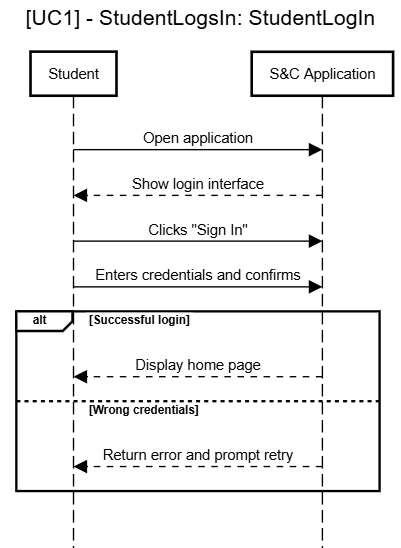
\includegraphics [width=.7\linewidth] {UC1.png}
    \caption{Student Login}
\end{figure}

\begin{figure} [H]
    \centering
    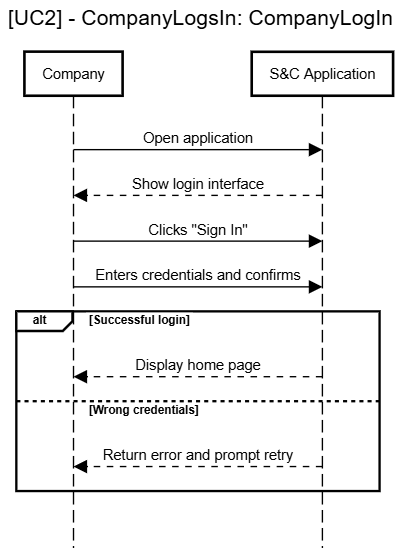
\includegraphics [width=.7\linewidth] {UC2.png}
    \caption{Company Login}
\end{figure}

\begin{figure} [H]
    \centering
    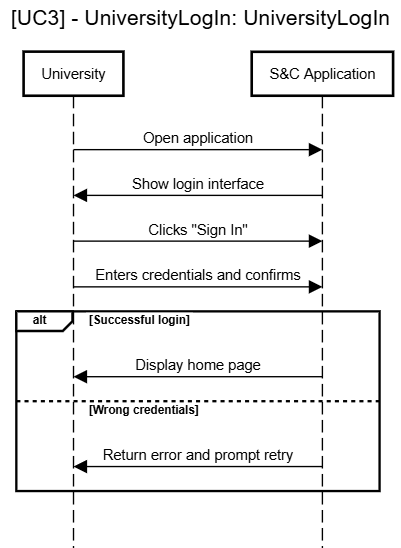
\includegraphics [width=.7\linewidth] {UC3.png}
    \caption{University Login}
\end{figure}

\begin{figure} [H]
    \centering
    
    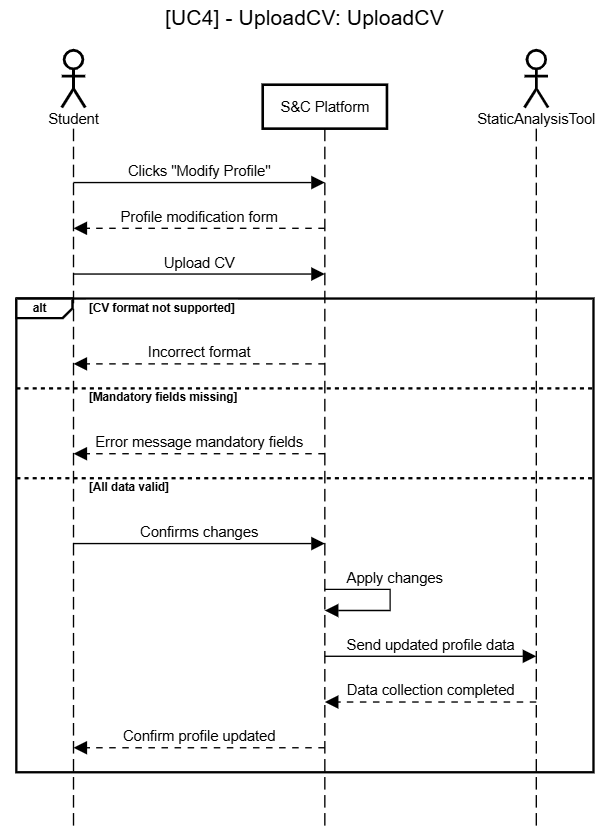
\includegraphics [width=.7\linewidth] {UC4.png}
    \caption{Upload CV}
\end{figure}

\begin{figure} [H]
    \centering
    
    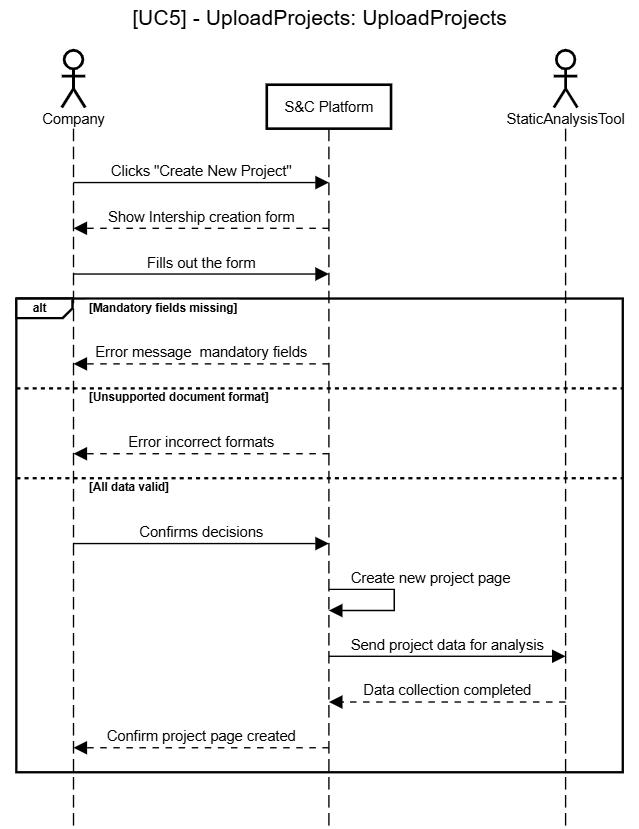
\includegraphics [width=.7\linewidth] {UC5.png}
    \caption{Upload Projects}
\end{figure}

\begin{figure} [H]
    \centering
    
    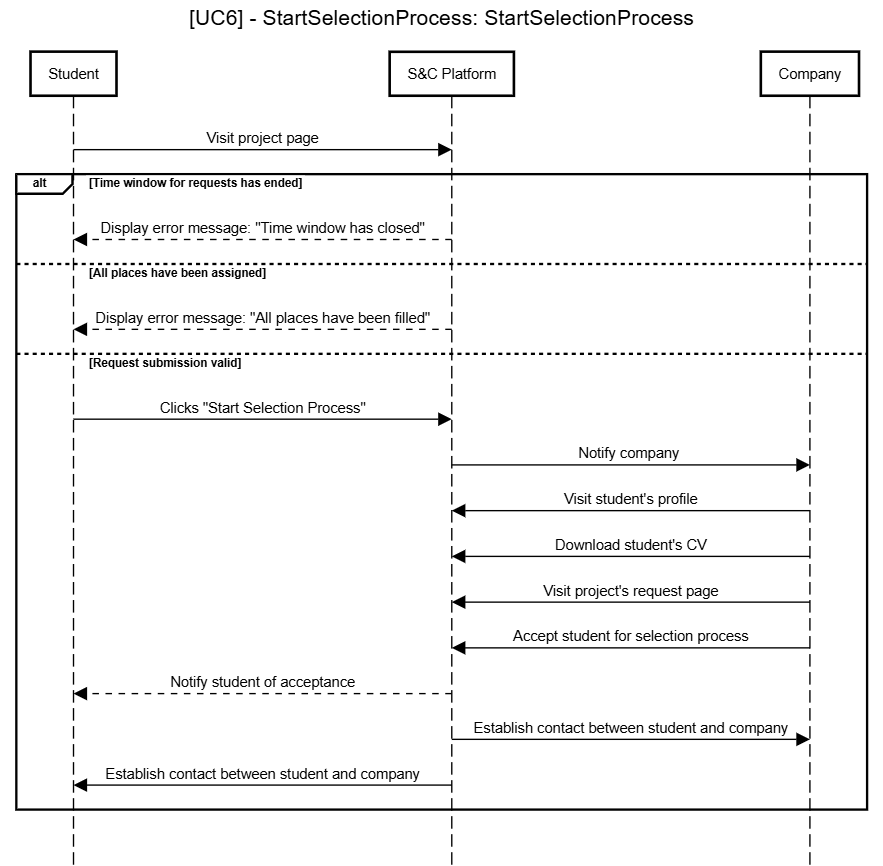
\includegraphics [width=.7\linewidth] {UC6.png}
    \caption{Start Selection Process}
\end{figure}

\begin{figure} [H]
    \centering
    
    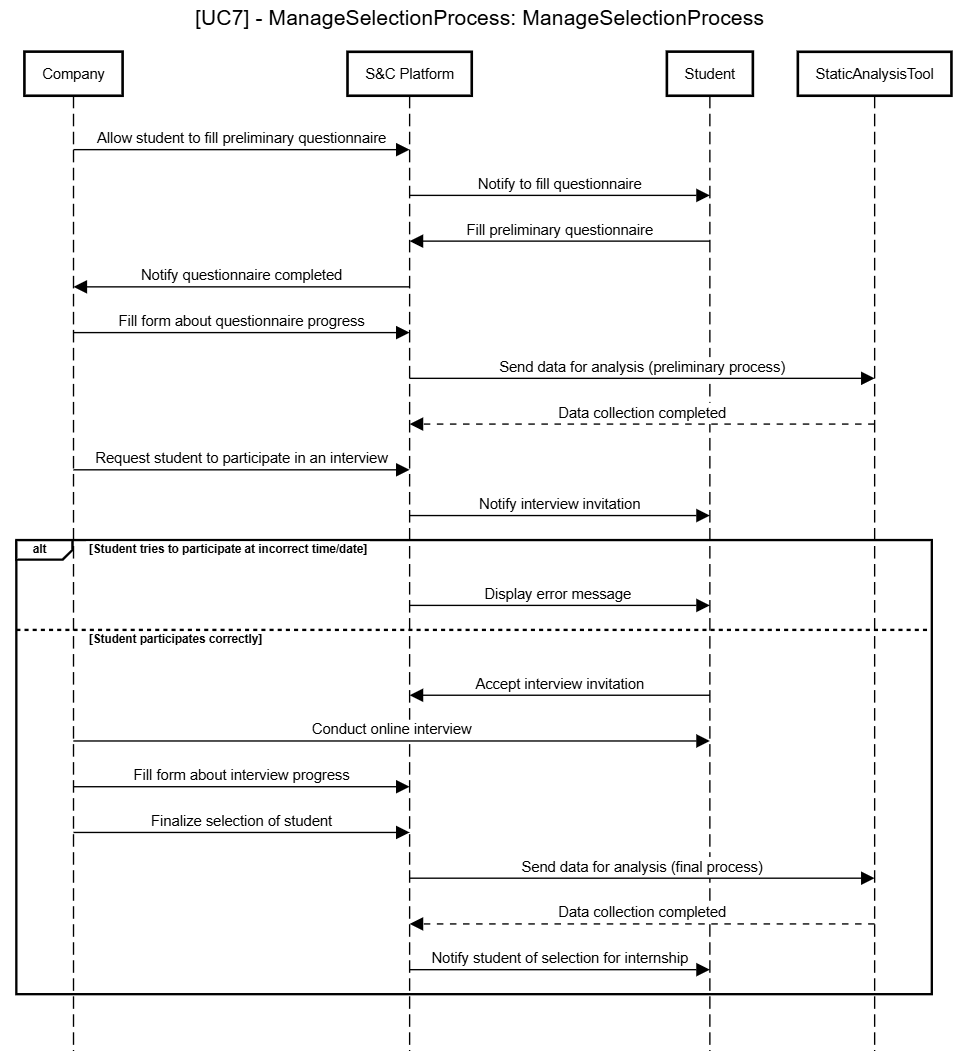
\includegraphics [width=.7\linewidth] {UC7.png}
    \caption{Manage Selection Process}
\end{figure}

\begin{figure} [H]
    \centering
    
    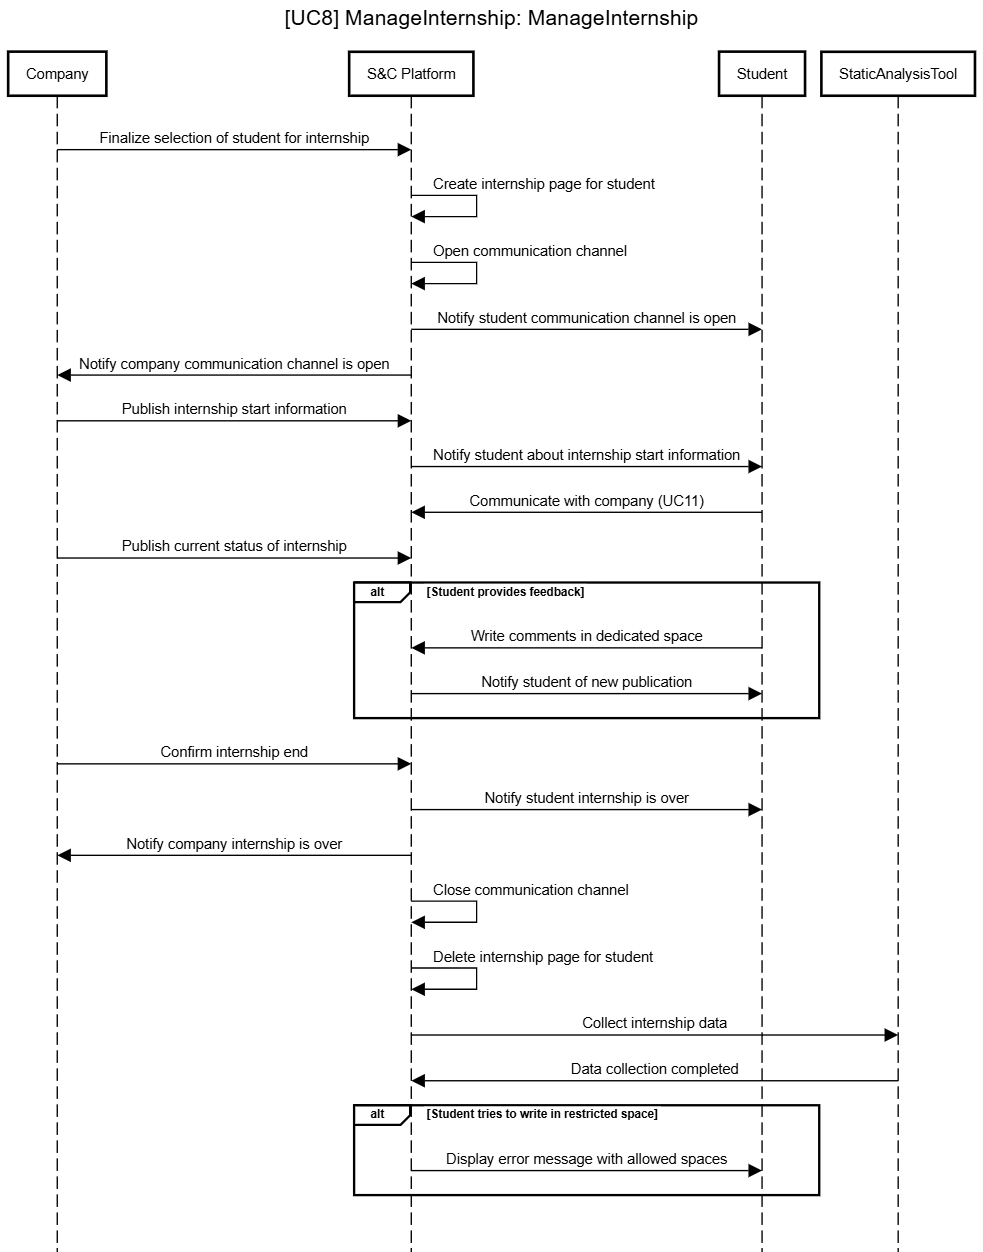
\includegraphics [width=.7\linewidth] {UC8.png}
    \caption{Manage Internship}
\end{figure}

\begin{figure} [H]
    \centering
    
    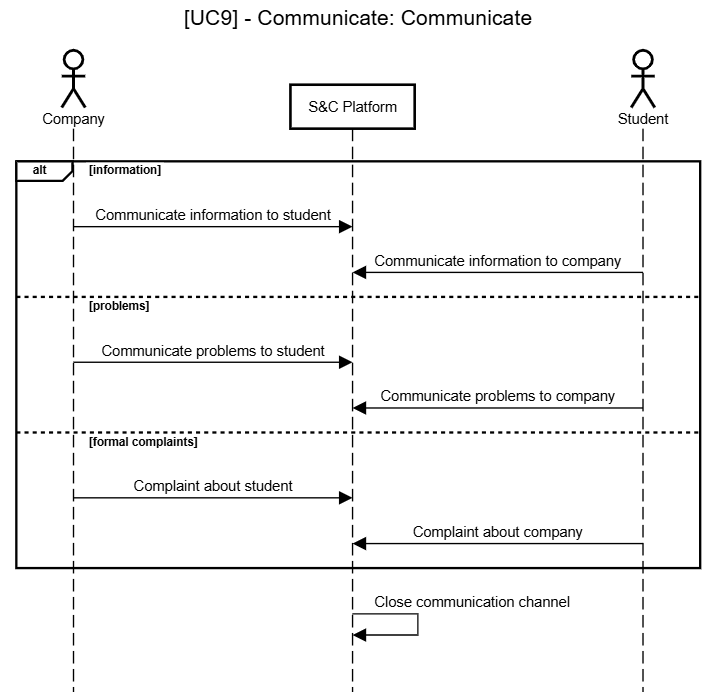
\includegraphics [width=.7\linewidth] {UC9.png}
    \caption{Communicate}
\end{figure}

\begin{figure} [H]
    \centering
    
    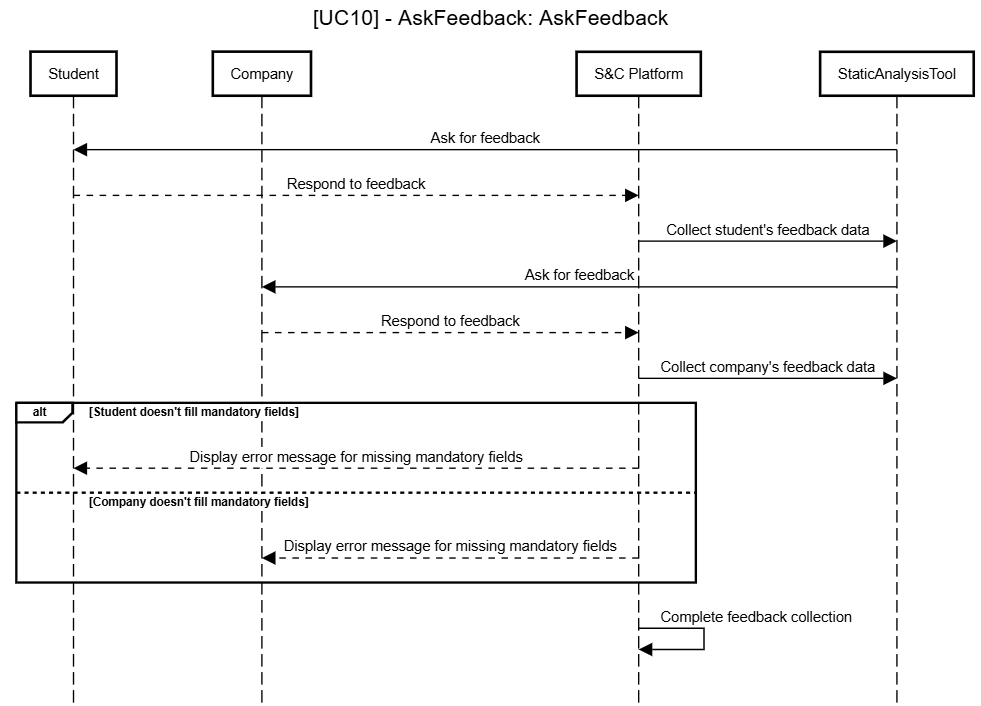
\includegraphics [width=.7\linewidth] {UC10.png}
    \caption{Ask Feedback}
\end{figure}

\begin{figure} [H]
    \centering
    
    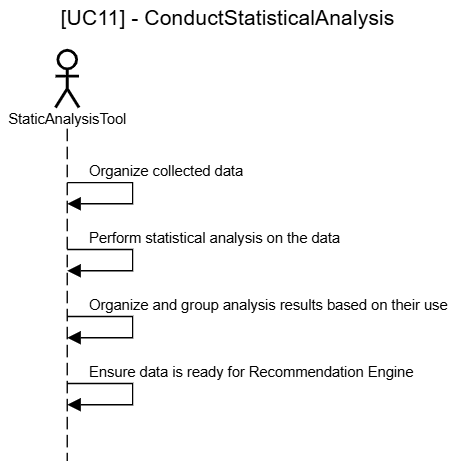
\includegraphics [width=.7\linewidth] {UC11.png}
    \caption{Conduct Statistical Analysis}
\end{figure}

\begin{figure} [H]
    \centering
    
    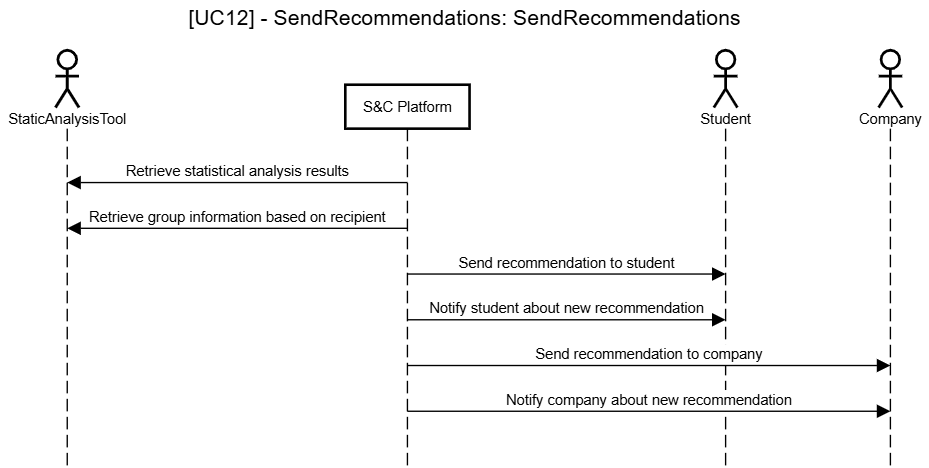
\includegraphics [width=.7\linewidth] {UC12.png}
    \caption{Send Reccommendations}
\end{figure}

\begin{figure} [H]
    \centering
    
    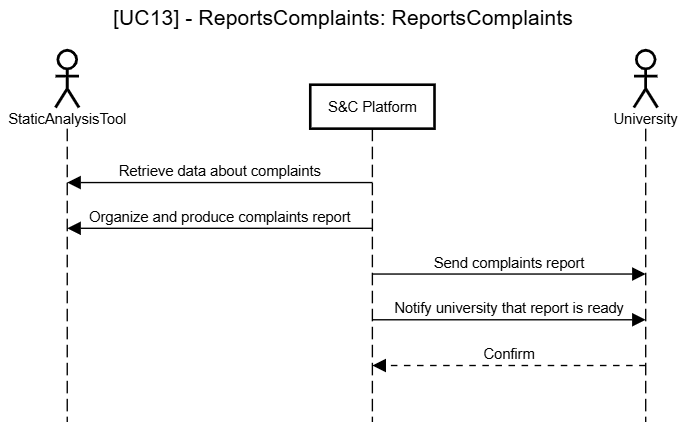
\includegraphics [width=.7\linewidth] {UC13.png}
    \caption{Reports Complaints}
\end{figure}

\begin{figure} [H]
    \centering
    
    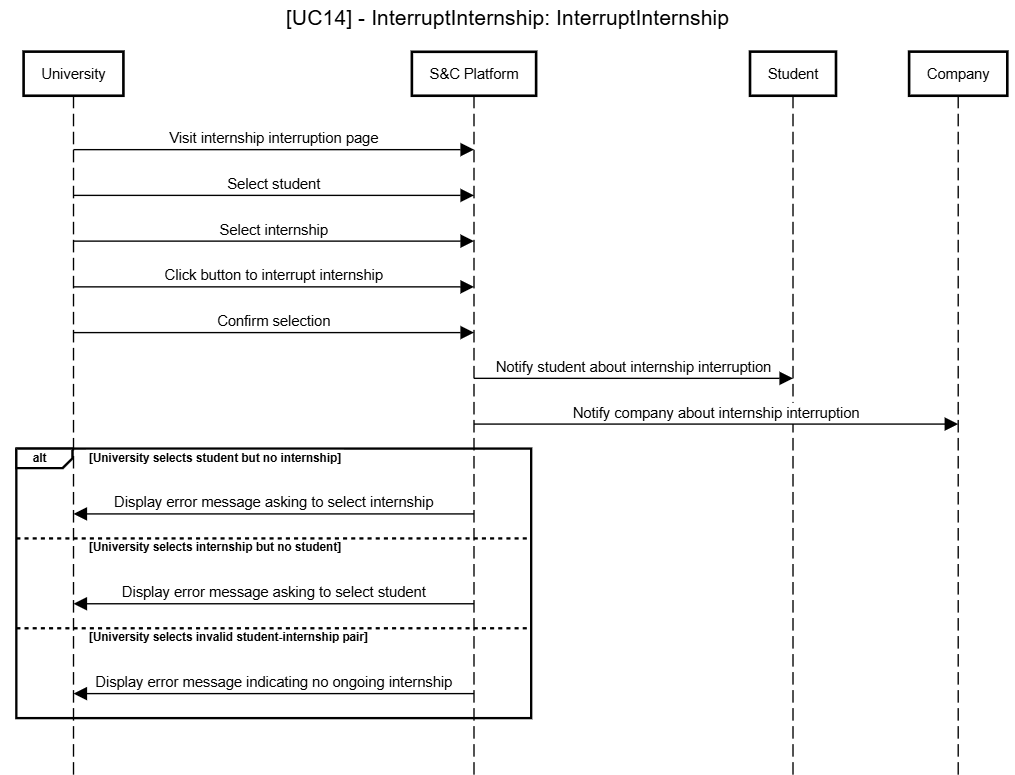
\includegraphics [width=.7\linewidth] {UC14.png}
    \caption{Interrupt Internship}
\end{figure}

\subsection{Activity Diagrams}
\subsection{Requirements Mapping}


\section{Performance Requirements}
\section{Design Constraints}

\section{Software System Attributes}

 % Specific Requirements
\chapter{Alloy}

In this section it is provided a representation of the world of CKB using the Alloy language. Every
run and every check are commented in order to guarantee a syntactical correct compilation of the
code: it is up to the reader to decide what to uncomment based on their will.

\lstinputlisting[language=alloy]{alloy_code.als}

\newpage
% //////////////////////////////
% ------------------------------
\section{Generated Worlds}
% ------------------------------
% //////////////////////////////

ciao % Alloy
\chapter{Effort Spent}
Time spent (mesured in hours) on every section of the RASD document by team member

\begin{longtable}{|>{\columncolor[HTML]{CFE2F3}}c|c|c|c|c|}
    \hline
    \textbf{Student} & \textbf{Introduction} & \textbf{Overall Description} & \textbf{Specific Requirements} & \textbf{Alloy}\\ \hline
    \endfirsthead
    \hline
    \textbf{Student} & \textbf{Introduction} & \textbf{Overall Description} & \textbf{Specific Requirements} & \textbf{Alloy}\\ \hline    \endhead
    \hline

    Simone & 0 & 0 & 0 & 0 \\ \hline
    Valeria & 0 & 0 & 0 & 0\\ \hline
    Toni & 0 & 0 & 0 &0 \\ \hline
\end{longtable} % Effort Spent
\chapter{Effort Spent} % References
% \chapter{Per fare prove}

Ciao ragazzi come va?


Questo lo ho aggiunto dopo.

Questo aggiunto dopo da VS code direttamente.


modifica in chimata

tabella tipo 1:


Tabella tipo 2:


%-------------------------------------------------------------------------
%	BIBLIOGRAPHY
%-------------------------------------------------------------------------

% \addtocontents{toc}{\vspace{2em}} % Add a gap in the Contents, for aesthetics
% \bibliography{Thesis_bibliography} % The references information are stored in the file named "Thesis_bibliography.bib"

%-------------------------------------------------------------------------
%	APPENDICES
%-------------------------------------------------------------------------

% \cleardoublepage
\addtocontents{toc}{\vspace{2em}} % Add a gap in the Contents, for aesthetics
% \appendix
% \chapter{Appendix A}
% If you need to include an appendix to support the research in your thesis, you can place it at the end of the manuscript.
% An appendix contains supplementary material (figures, tables, data, codes, mathematical proofs, surveys, \dots)
% which supplement the main results contained in the previous chapters.

% \chapter{Appendix B}
% It may be necessary to include another appendix to better organize the presentation of supplementary material.
\printglossary[type=\acronymtype]

% LIST OF FIGURES
% \listoffigures

% LIST OF TABLES
% \listoftables

% % LIST OF SYMBOLS
% % Write out the List of Symbols in this page
% \chapter*{List of Symbols} % You have to include a chapter for your list of symbols (
% \begin{table}[H]
%     \centering
%     \begin{tabular}{lll}
%         \textbf{Variable} & \textbf{Description} & \textbf{SI unit} \\\hline\\[-9px]
%         $\bm{u}$ & solid displacement & m \\[2px]
%         $\bm{u}_f$ & fluid displacement & m \\[2px]
%     \end{tabular}
% \end{table}

% ACKNOWLEDGEMENTS
% \chapter*{Acknowledgements}
% Here you may want to acknowledge someone.

% \cleardoublepage

\end{document}
